\documentclass[12pt]{article} 
\usepackage[pdftex]{graphicx}
\usepackage{natbib} 
\usepackage{color}
\usepackage{amsmath} 
\usepackage{amssymb} 
\usepackage{verbatim}
\usepackage{mathpazo} 
\usepackage{setspace}
\usepackage{multirow}
\usepackage{fullpage}
\usepackage{lscape}
\usepackage{fancyhdr}
\usepackage[normalem]{ulem} 
\usepackage{hyperref}
\usepackage[parfill]{parskip}
\usepackage{graphicx}
\usepackage{rotating}
\usepackage{textcomp}
\hypersetup{colorlinks=true, linkcolor=black, citecolor=black}
\RequirePackage{lineno}

\newcommand{\flagged}[1] {
  \textcolor{blue}{#1}
}

\def\title{Improving the efficiency of occupancy models (something
  more interesting sounding?)}
\def\author{Lauren C.\ Ponisio$^{1,2,3}$, Nicholas Michaud$^1$, Perry de
  Valpine$^1$ (Daniel and Chris?)}

\def\runninghead{Occupancy model efficiency}
\def\keywords{NIMBLE, Markov chain Monte Carlo, latent states, block
  sampling, dynamic occupancy, mutli species occupancy, spatial
  occupancy, JAGS }

\def\extras{
  \begin{itemize}
  \item Submitted as a Standard paper
  \item Abstract word count: 
  \item Main text word count: 
  \item Number of references: 
  \item Number of figures:
  \end{itemize}
}

\def\affiliation{
  \begin{enumerate}
  \item Department of Environmental Science, Policy, and Management\\
    University of California, Berkeley\\
    130 Mulford Hall\\
    Berkeley, California, USA\\
    94720\\
  \item Berkeley Institute for Data Science (BIDS)\\
    University of California, Berkeley\\
    190 Doe Library \\
  \item Department of Entomology\\
    University of California, Riverside\\
    417 Entomology Bldg.\\
    Riverside, California, USA\\
    92521\\
  \end{enumerate}
}

\newcommand{\mstitlepage}{
  \paragraph{Running head:} \textsc{\runninghead}
  % \parindent=0pt
  \begin{center}%
    {\LARGE \title \par}%
    \vskip 3em%
    {\large
      \lineskip .75em%
      \begin{tabular}[t]{c}%
        \author
      \end{tabular}\par}%
    \vskip 1.5em%
  \end{center}\par
  \affiliation
}
\clearpage

\begin{document}

\mstitlepage
\doublespacing
\linenumbers
\clearpage

\begin{abstract}  
  \begin{enumerate}
  \item Something expressing the sentiment: occupancy models are
    everywhere, but model fitting and assessment are extremely
    computationally intensive
  \item Because models are so computationally intensive, users often
    forgo model assessment (determining if a model provides an
    adequate fit to a particular dataset) and model selection
    (choosing the best model out of a set of models) --- methods that
    generally involve simulating from and refitting the model
    iterativly.
  \item Using the open source modeling software NIMBLE, we develop
    combined computational approaches including user-defined and
    automatic blocking of parameters for MCMC, filtering over latent
    states, and customized MCMC samplers for specific parameters to
    improve efficiency. We test these approaches using three
    representative occupancy models of varying levels of complexity
    including a single species model with spatial auto-correlation, a
    single species dynamic (multi-season) model, and a multi-species
    model. We also develop and implement methods for calculating
    calibrated predictive posterior $p$-values to assess model fit and
    cross validation for model selection within NIMBLE.
  \item These computation approaches lead to an improvement in MCMC
    sampling efficiency over, particularly with models including
    random effects (maybe?). (more results once they are available)
  \item \textit{Implications:} Ours results highlight the need for
    more customizable approaches to MCMC to fit and assess
    hierarchical models in order to ensure occupancy and other
    hierarchical models are accessible to practitioners. By
    implementing MCMC procedures and model assessment and selection
    techniques in open source software, we have made progress toward
    this aim.
  \end{enumerate}
\end{abstract}

\keywords

\clearpage

\section*{Introduction}
\label{sec:introduction}

Estimating the proportion of sites occupied by a species is common
challenge for many sub-disciplines in ecology and evolution including
meta-population, endangered species and invasion biology. Greater
acceptance of the biases introduced by imperfect detection has lead to
the development and proliferation of occupancy models where the
occurrence of a species at a site is modeled as a latent state layered
underneath a detection process \citep[e.g.,][]{mackenzie-2006,
  royle-2007-1813}. Now only a little over a decade after occupancy
models were introduced to ecology, they are being used to model the
occurrence of everything from bees \citep{mgonigle-2015-x} to tigers
\citep{hines2010tigers} in an endless variety of complexity.

Occupancy models are part of a larger class of models known as Hidden
Markov Models. In discrete Hidden Markov Models like occupancy models
where a species is either present or absent from a site, likelihood
calculation involves summing over the distribution of latent
states. Because estimating the effect of explanatory variables on site
occupancy or shared variation in occupancy across species is often of
greatest interest to biologists \citep[e.g.,][]{iknayan2014detecting},
the Hidden Markov Model is often embedded within a hierarchical
model. In such cases, practitioners generally rely on Markov chain
Monte Carlo (MCMC) to perform a Bayesian analysis. Standard MCMC
software will include the latent state variables in MCMC sampling
\citep[e.g.,][]{plummer-2003-jags, winbugs, openbugs}. Such models are
computationally intensive, and large models requiring hundreds or
thousands of dimensions which require MCMC can be intractable.

In addition, fitting these models is such a challenge that users often
forgo any additional computation to asses model fit. A common idea
behind evaluating whether a model provides an adequate fit to a
dataset is that if data is simulated from the model, the simulated
data should resemble the observed data. This is the basis of posterior
predictive $p$-values, which compare the distribution of summary
statistics calculated from simulated datasets to the observed
statistic. Posterior predictive $p$-values alone, however, often fail
to reject poor-fitting models \citep{bayarri-berger-00,
  robins-etal-00, hjort-etal-06}. Methods for correcting posterior
predictive $p$-values for better performance by refitting the model
via MCMC iterativly have been proposed \citep[e.g., calibrated
posterior predictive $p$-values, ][]{hjort-etal-06}, but no methods
are available in open source software. In addition, given fitting an
occupancy model just once can be a time consuming task, efficient
methods for MCMC are necessary to ensure methods for assessment are
feasible for these models.

Beyond assessing the fit of a model, choosing between models is one of
the most widely used applications of statistics by
practitioners. Though many methods for Bayesian model selection have
been developed \citep{hooten2014guide}, but they, like model
assessment, are computationally intensive. For example,
cross-validation, one of the most fundamental procedures in model
selection, requires iterativly re-fitting the model. A typical need
for model selection arises when a practitioner is choosing whether to
include a specific layer of hierarchy (i.e., random effect). This is
often the case with so called ``multi-species'' occupancy models,
where the occupancy of many species is estimated simultaneously in a
model with a random effect of species \citep[reviewed in,
][]{iknayan2014detecting}. Ecologists are often interested in whether
there is some variability in the response of species to an explanatory
variable such that a random effect of species accounts for that
variability \citep{pacifici2014guidelines}. Currently, the Deviance
Information Criteria (DIC), originally derived to mimic AIC for
Bayesian, non-hierarchical models, is now commonly used by scientists
to evaluate hierarchical models. Though the limitations of DIC for
hierarchical model selection are widely recognized by statisticians
\citep{celeux2006deviance, hooten2014guide}, because it is built into
open-source software such as WinBUGS, it can be used uncritically by
practitioners. Readily available and theoretically sound alternative
methods are thus greatly needed.

Luckily, methods to improve MCMC efficiency of Hidden Markov Models
have been developed such filtering over latent states to calculate
model likelihoods in order to limit MCMC sampling to top-level
parameters dynamic blocking or parameters
\citep{turek2016efficient}. A synergistic strategy is to assign
specific MCMC samplers to different parameters depending on the nature
of those nodes (i.e., discrete versus continuous). Though these
methods are available in isolation in application-specific software,
they cannot be used in combination for any arbitrary model structure.

Using the open source modeling software NIMBLE, we develop combined
computational approaches including user-defined and automatic blocking
of parameters for MCMC, filtering over latent states, and customized
MCMC samplers for specific parameters to improve efficiency. We test
these approaches using three representative occupancy models of
varying levels of complexity including a single species model with
spatial auto-correlation, a single species dynamic (multi-season)
model, and a multi-species model. We also develop and implement
methods for calculating calibrated predictive posterior $p$-values to
assess model fit and cross validation for model selection within
NIMBLE. 


\section*{Materials \& Methods}
\label{sec:methods}
\subsection*{Computational approaches}

\subsubsection*{Single species, single season occupancy model with
  spatial auto-correlation}
The first model we explore is a single species, single season
occupancy model accounting for spatial auto-correlation. We let
$z_{i}$ denote the true occupancy of a species at site $i$.  We then
let $x_{i,j}$ indicate whether the species was ($x_{i,j}=1$), or was
not detected ($x_{i,j}=0$) in the $j^{\mathrm{th}}$ visit to site $i$.
We assumed that occupancy at the $i^{\mathrm{th}}$ site is a Bernoulli
random variable $z_{i} \sim \mathrm{Bern}(\psi_{i})$ with probability
$\psi_{i}$.  We included the effect of an arbitrary covariate (e.g.,
elevation) on site occupancy. To model the spatial auto-correlation in
occupancy between sites, we assume the co-variance between sites $Y_i$
and $Y_j$ is a function of distance between $p_i$ and $p_j$. We
computed the probability of occupancy at site $i$
%
\begin{equation}
  \begin{split}
    \label{eq:spatial}
    \mathrm{logit}(\psi_{i}) &=
    \alpha + \beta*elevation_i + \rho_i\hspace{0.2em}\\
    \rho_i &\sim MVN(0, {Cov}(Y_i,Y_j)) \hspace{0.2em}\\
    {Cov} (Y_i,Y_j) &= \sigma^2exp^{(-\lambda\|p_i-p_j\|)} \hspace{0.2em}.\\
  \end{split}
\end{equation}
%

Where $\lambda$ is the exponential decay constant and $\sigma^2$ is
\flagged{SOMETHING...}

We simulate data for this model and then fit it using the default
settings for NIMBLE and JAGS. \flagged{To improve efficiency of this
  model...}

We implemented a procedure to calculate calibrated posterior
predictive $p$-values \citep[CPPP, ][]{hjort-etal-06} to assess the
fit of the model to the data. After the parameters have been fit to
the model, a sample of the posterior is used to simulate data from the
model. A discrepancy measure, which we chose to be the model
likelihood, is then calculated, and the posterior $p$-value is the
number of simulated $p$-values that fall below the observed. To
``calibrate'' the distribution of posterior $p$-values, the MCMC is
rerun on the simulated data to refit the model. If the CPPP $< 0.05$,
the model is rejected as having an adequate fit to the data
\citep{hjort-etal-06}.

\subsubsection*{Single species, multi season (dynamic) occupancy
  model}
\label{sec:ssms}

The second model we examine is a relatively simple single species
occupancy model over multiple seasons \citep{Royle2007}. We let
$z_{i,j}$ denote the true occupancy of a species in year $j$ at site
$i$.  We assumed that occupancy at the $i^{\mathrm{th}}$ site in the
$j^{\mathrm{th}}$ year is a Bernoulli random variable $z_{i,j} \sim
\mathrm{Bern}(\psi_{i,j})$.

Letting $\phi_{i,j}$ denote the probability the species persists at
site $i$ from years $j$ to $j+1$ (provided it was present at site $i$
in year $j$, $z_{i,j}=1$) and $\gamma_{i,j}$ denote the probability
that site $i$ is colonized in year $j+1$ (provided it was not present
at site $i$ in year $j$, $z_{i,j}=0$), we then computed the
probability of occupancy at site $i$ in subsequent years as
%
\begin{equation}
  \label{eq:mutliseason}
  \psi_{i,j+1} =
  \phi_{i,j} * z_{i,k} + \gamma_{i,j} * (1-z_{i,j})\hspace{0.2em}.
\end{equation}
%

We then let $x_{i,j,k}$ indicate whether that species was
($x_{i,j,k}=1$) or was not detected ($x_{i,j,k}=0$) in the
$k^{\mathrm{th}}$ visit to site $i$ in year $j$. We assume detection
was distributed according to be a Bernoulli random variable such that
$x_{i,j,k} \sim \mathrm{Bern}(p_{j}*z_{i,j})$, where $p_{j}$ is the
probability that the species was detected at site $i$ in the
$j^{\mathrm{th}}$ year, given that it was present.

As with the spatial occupancy model, we first simulate data for this
model and then fit it using the default settings for JAGS and NIMBLE
where all model parameters and latent states undergo MCMC sampling
(``NIMBLE-latent'' and ``JAGS-latent'', respectively). Following
\cite{Royle2007, kery-schaub-11}, we use uninformative,
$\mathrm{Unif}(0,1)$ priors for all parameters.

Next, to improve efficiency, using NIMBLE we filter over latent states
to calculate model likelihoods in order to limit MCMC sampling to
top-level parameters (``filter''). \flagged{Do we want to write out
  the likelihood?)} We then use two additional computational
approaches to improve the efficiency of this model 1) dynamic blocking
of the parameters \citep[``filter + autoblocking'',
][]{turek2016efficient}, and 2) a custom MCMC specification where
slice samplers \citep{neal-03} are used for all parameters (``filter +
slice''). Slice samplers are a class of methods that sample from a
target distribution by using that fact that samples from any
distribution can be obtained by sampling uniformly from the area under
that distribution's probability density function curve.  The
horizontal coordinates of these uniform samples will provide samples
from the distribution of interest. Slice samplers have been shown to
perform well in situations where choosing a tuning parameter for a
Metropolis algorithm is difficult. When used to sample from the
posterior distribution of a univariate parameter, a slice sampler
proceeds at each iteration by first choosing a vertical coordinate
sampled uniformly between 0 and the height of the density curve at the
parameter value from the previous iteration.  Then, a horizontal
coordinate is chosen uniformly from the set of all possible parameter
values whose density is at least as great as the chosen vertical
coordinate.  \flagged{other options we want to present?}

As with the spatial model, we use calibrated posterior predictive
$p$-values \citep{hjort-etal-06} to assess the fit of the model to
the data.

\subsubsection*{Multi species, single season occupancy model}
\label{sec:msss}

The last model we analyze is a multi-species, single season occupancy
model examining the effect of wildlife management and habitat
characteristics on bird communities \citep{zipkin2010multi}. The
species-specific coefficients for the effect of basal tree area,
understory foliage and deer management where bound together by a
common distribution with an estimated variance.  For species $i$, we
let $z_{i,j}$ denote its true occupancy state at site $j$. We assumed
that the occupancy of the $i^{\mathrm{th}}$ species at the
$j^{\mathrm{th}}$ site is a Bernoulli random variable $z_{i,j} \sim
\mathrm{Bern}(\psi_{i,j})$.  We then let $x_{i,j,k}$ indicate whether
species $i$ was ($x_{i,j,k}=1$) or was not detected ($x_{i,j,k}=0$) in
the $k^{\mathrm{th}}$ visit to site $j$. We also assumed that
detection was distributed according to be a Bernoulli random variable
such that $x_{i,j,k} \sim \mathrm{Bern}(p_{i}*z_{i,j})$, where $p_{i}$
is the probability that the $i^{\mathrm{th}}$ species was
detected. Both site occupancy and detection were influence by habitat
and survey characteristics \citep{zipkin2010multi}. Specifically,
occurrence depended on the study area (CATO, Ind=1, or FCW, Ind=0), the
basal tree area (BA) and the understory foliage cover (UFC). The
species-specific occupancy probabilities are modeled as

\begin{equation}
  \begin{split}
    \label{eq:multispecies}
    \mathrm{logit}(\psi_{i,j}) &= uCATO_i(Ind_j) + uFCW_i(1-Ind_j) +
    \alpha1_iUFC_j + \alpha2_iUFC^2_j + \alpha3_iBA_j +
    \alpha4_iBA^2_j \\
     \alpha1 &\sim N({\mu}_{\alpha1}, \sigma^2_{\alpha1})\\
     \alpha2 &\sim N({\mu}_{\alpha2}, \sigma^2_{\alpha2})\\
     \alpha3 &\sim N({\mu}_{\alpha3}, \sigma^2_{\alpha3})\\
     \alpha4 &\sim N({\mu}_{\alpha4}, \sigma^2_{\alpha4})
   \hspace{0.2em}
  \end{split}
\end{equation}

Similarly, detection depended on survey location and the date:

\begin{equation}
  \begin{split}
    \label{eq:multispecies_detection}
    \mathrm{logit}(p_{i,j,k}) &= vCATO_i(Ind_j) + vFCW_i(1-Ind_j) +
    \beta1_idate_j + \beta2_idate^2_j\\
     \beta1 &\sim N({\mu}_{\beta1}, \sigma^2_{\beta1})\\
     \beta2 &\sim N({\mu}_{\beta2}, \sigma^2_{\beta2})\\
    \hspace{0.2em}
  \end{split}
\end{equation}

We first fit the using the default settings for JAGS and NIMBLE where
all model parameters and latent states undergo MCMC sampling
(``NIMBLE-latent'' and ``JAGS-latent'', respectively). We use
uninformative priors, $\mathrm{Norm}(0,1000)$ for the means of the
distributions of the hyperparameters and $\mathrm{Unif}(0,100)$ the
variances.

To improve the efficiency of this model, we first filtered over latent
states to calculate model likelihoods in order to limit MCMC sampling
to top-level parameters (``filter''). We also vectorized all
calculations that would have require for loops in JAGS. \flagged{Do we
  want to write out the likelihood?)} We then applied two approaches
to speed sampling of the top-level parameters 1) dynamic blocking of
the parameters \citep[``filter + autoblocking'',
][]{turek2016efficient}, and 2) a custom blocking scheme where the
parameters of each species are blocked together with adaptive random
walk MCMC (``Filter + species blocking''). Random walk Metropolis
algorithms \citep{metropolis1953equation} sample from the posterior
distribution of a parameter of interest by first proposing a new
parameter value from a normal proposal distribution centered at the
current value, and then deciding whether to accept or reject the
proposed value via the Metropolis ratio.  Although common, standard
univariate or multivariate normal proposal distributions can prove to
be inefficient at sampling for models in which parameters are highly
correlated.  Adaptive random walk Metropolis sampling
\citep{haario98anadaptive} allows the correlation structure of the
posterior distribution of blocks of parameters to be used to produce
better proposals.  For an occupancy model where parameters are highly
correlated within species, this can provide much more efficient
sampling than a non-adaptive Metropolis algorithm.

We also use calibrated posterior predictive $p$-values
\citep{hjort-etal-06} to assess the fit of the model to the data.  In
multi-species occupancy models, practitioners are often interested in
determining whether a model including a species random effect for
explanatory variables is a better fit than a model without the random
effect. We implemented a cross-validation procedure for this model
where the detection data for species is left out, the model refitted,
and the fitted model used to predict the occurrence of that
species. The predictive error of the model included a random effect of
species is then compared to a model where no species random effects
were included.

% a subset of the data ($y_k$) if excluded from model fitting, the the
% fitted model is used to predict $y_k$. The prediction error is
% summarized by comparing the simulated $y_k$ to the true $y_k$.

\section*{Results}
\label{sec:results}

\subsubsection*{Multi species, single season occupancy model}
\label{sec:msss-res}

\subsubsection*{Single species, single season occupancy model with
  spatial auto-correlation}
\label{sec:sp-res}

\subsubsection*{Single species, multi season (dynamic) occupancy
  model}
\label{sec:ssms-res}

\section*{Discussion}
\label{sec:discussion}

\section*{Acknowledgments}
\label{sec:acknowledge}

\bibliographystyle{mee}

\bibliography{refs}


\begin{figure}
  \centering
  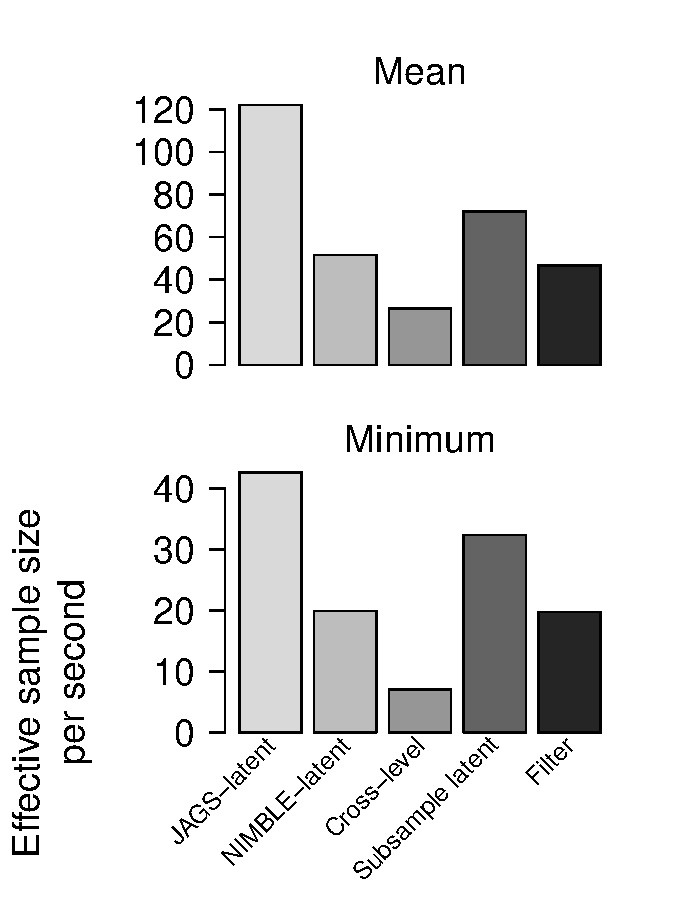
\includegraphics[width=.8\textwidth]{../../../saved/SingleSpp-MultiSea/figures/comparisons/SingleSpp-MultiSeaBar.pdf}
  \caption{The mean and minimum efficiency of different MCMC samplers
    for the single species, multi season occupancy model.}
  \label{fig:ss-ms-eff}
\end{figure}
\clearpage


\begin{sidewaysfigure}
  \centering
  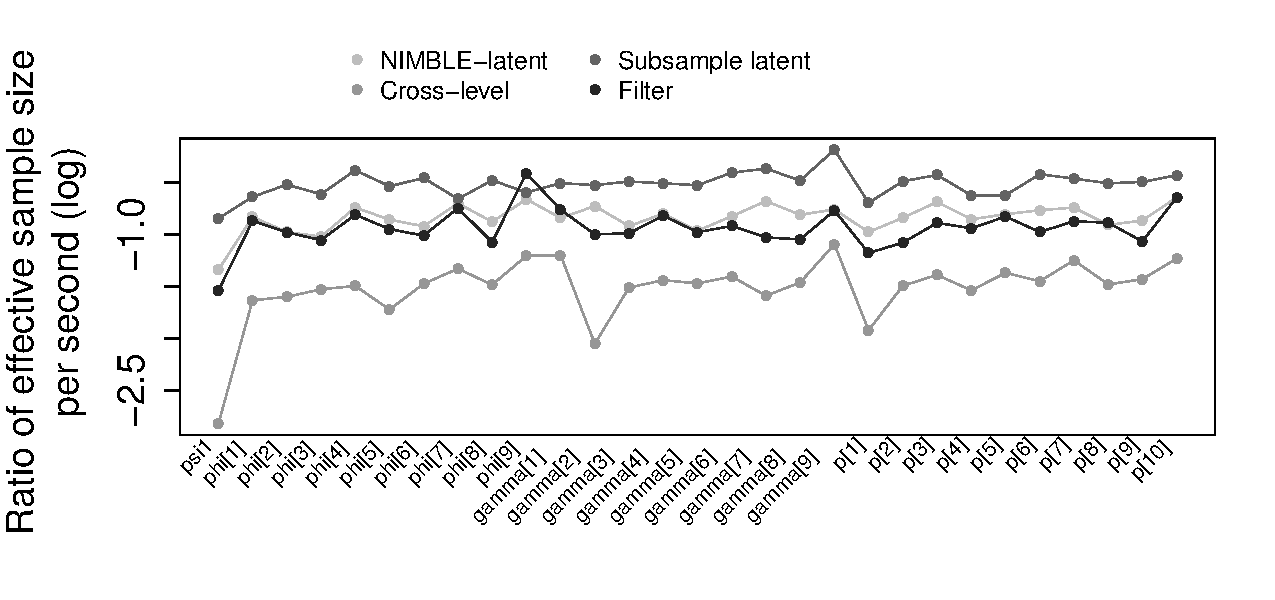
\includegraphics[width=.8\textwidth]{../../../saved/SingleSpp-MultiSea/figures/comparisons/SingleSpp-MultiSeaDiffs.pdf}
  \caption{The log ratio of the NIMBLE samplers in comparison to the
    JAGS sampler for the single species, multi season occupancy
    model.}
  \label{fig:ss-ms-eff}
\end{sidewaysfigure}
\clearpage


\begin{figure}
  \centering
  \includegraphics[width=.8\textwidth]{../../../saved/multiSpp-singleSea/figures/comparisons/MultiSpp-SingleSeaBar.pdf}
  \caption{The mean and minimum efficiency of different MCMC samplers
    for the multi species, single season occupancy model.}
  \label{fig:ms-ss-eff}
\end{figure}
\clearpage


\begin{sidewaysfigure}
  \centering
  \includegraphics[width=.8\textwidth]{../../../saved/multiSpp-singleSea/figures/comparisons/MultiSpp-SingleSeaDiffs.pdf}
  \caption{The log ratio of the NIMBLE samplers in comparison to the
    JAGS sampler for the multi species, single season occupancy
    model.}
  \label{fig:ms-ss-eff}
\end{sidewaysfigure}
\clearpage



\end{document}

%%% Local Variables:
%%% mode: latex
%%% TeX-PDF-mode: t
%%% End:
